\section{INTRODUCTION}\label{Sec:intro}
This is an introduction to $\LaTeX$ for the COMP0219 course.  The basic $\LaTeX$ tricks you may want are the following.  First, make sure that you write all your text in the main.tex.  Whenever you want to check the .pdf file, press the PDF button on the left sidebar and click: Recompile.  Secondly, you should be able to include figures and images in your document, which is done as follows (give always a label):

In Fig.~\ref{Fig:universe} we show a picture of the universe!

\begin{figure}[ht!]
  \centering
  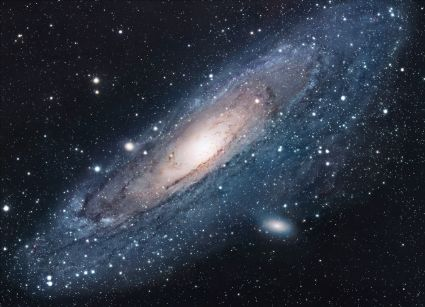
\includegraphics[scale=1.7]{figures/universe.jpg}
  \caption{The Universe}
  \label{Fig:universe}
\end{figure}